\documentclass{beamer}
\mode<presentation>
\usetheme{CambridgeUS}
\usepackage[russian]{babel}
\usepackage[utf8]{inputenc}
\usepackage[T2A]{fontenc}
\usepackage{sansmathaccent}
\usepackage{alltt}
\linespread{0.8}
\usepackage{minted}

\pdfmapfile{+sansmathaccent.map}
\title[Язык C]{Составные (агрегированные) типы данных}
\author{Наумов Д.А., доц. каф. КТ}
\date[10.09.2020] {Операционные системы и системное программное обеспечение, 2020}

\begin{document}

%ТИТУЛЬНЫЙ СЛАЙД
\begin{frame}
  \titlepage
\end{frame}
  
%СОДЕРЖАНИЕ ЛЕКЦИИ
\begin{frame}
  \frametitle{Содержание лекции}
  \tableofcontents  
\end{frame}

\section{Массивы}

\begin{frame}{Массивы}
    \textbf{Массив} -- это набор переменных одного типа, имеющих одно и то же имя. Доступ к конкретному элементу массива осуществляется с помощью \textbf{индекса}. 
    
    \medskip
    
    В языке С все массивы располагаются в отдельной непрерывной области памяти. Первый элемент массива располагается по самому меньшему адресу, а последний — по самому большому. В языке C массивы и указатели тесно связаны. 
    \medskip
    Объявление массива:
    \mint{c}|<<ElementsType>> <<ArrayName>>[<<ElementsCount>>];|
    \medskip
    Массив целых чисел длиной 10 элементов:
    
    \mint{c}|int a[10];|
    \medskip
    По сути, это блок из десяти последовательных объектов с именами 
    
    \mint{c}|a[0], a[1], ..., a[9];|
    \medskip
    Запись \texttt{a[i]} обозначает i-й элемент массива. Индексация элементов массива в языке C всегда начинается с нуля.
\end{frame}

\begin{frame}{Представление массивов в памяти}
    Объем памяти, необходимый для хранения массива, непосредственно
    определяется его типом и размером. Для одномерного массива количество байтов памяти вычисляется следующим образом:
    
    \begin{alltt}
    количество\_байтов = sizeof(базовый\_тип) × длина\_массива
    \end{alltt}
    
    Во время выполнения программы на С не проверяется ни соблюдение
    границ массивов, ни их содержимое. В область памяти, занятую массивом, может быть записано что угодно, даже программный код. 
    
    \medskip
    
    Программист должен сам, где это необходимо, ввести проверку границ индексов. Элементы одномерного массива хранятся в непрерывной области памяти в порядке индексации. Ниже показано, как хранится в памяти массив \texttt{а}, начинающийся по адресу 1000 и объявленный как \texttt{char a[8]}:
    
    \begin{alltt}
    \begin{tabular}{c c c c c c c c c}
    Элемент & a[0] & a[1] & a[2] & a[3] & a[4] & a[5] & a[6] & a[7] \\

    Адрес &  1000 & 1001 & 1002 & 1003 & 1004 & 1005 & 1006 & 1007
    \end{tabular}
    \end{alltt}
\end{frame}

\begin{frame}[fragile]{Пример}
    Следующий пример программы компилируется без ошибки, однако при выполнении происходит нарушение границы массива \texttt{count} и разрушение соседних участков памяти:
    \medskip
    \begin{minted}{c}
    
    int count[10], i;
    /* здесь нарушена граница массива count */
    for(i=0; i<100; i++)
        count[i] = i;
    
    \end{minted}
    \medskip
    Что произойдет при запуске такой программы?
\end{frame}

\begin{frame}[fragile]{Двухмерные массивы}
    Стандартом С определены многомерные массивы. Простейшая и самая распространенная форма многомерного массива - двухмерный массив. 
    \medskip
    Двухмерный массив - это массив одномерных массивов. Объявление двухмерного массива \texttt{d} с размерами 10 и 20 выглядит
    следующим образом:

    \medskip
    \begin{minted}{c}
    
    int d[10][20];
    
    \end{minted}
    \medskip
    В языке С каждый индекс заключен в свои квадратные скобки. 
    \medskip
    
    Аналогично обращению к элементу одномерного массива, обращение к элементу с индексами 1 и 2 двухмерного массива \texttt{d} выглядит так:
    
    \begin{alltt}
    d[1][2]
    \end{alltt}
\end{frame}

\begin{frame}{Инициализация массивов}
    В языке С массивы при объявлении можно инициализировать. Общая
    форма инициализации массива аналогична инициализации переменной:
    
    \begin{alltt}
    тип имя\_массива[размер1]...[размерN] = {список\_значений};
    \end{alltt}
    \begin{itemize}
        \item \texttt{Список\_значений} представляет собой список констант, разделенных запятыми. 
        \item Типы констант должны быть совместимыми с типом массива. 
        \item Первая константа присваивается первому элементу массива, вторая - второму и так далее. 
        \item После закрывающейся фигурной скобки точка с запятой обязательна.
    \end{itemize}
    
    В следующем примере массив целых из 10 элементов инициализируется числами от 1 до 10:
    
    \begin{alltt}
    int i[10] = \{1, 2, 3, 4, 5, 6, 7, 8, 9, 10\};
    \end{alltt}
    
    Здесь элементу \texttt{i[0]} присваивается 1, a \texttt{i[9]} - 10.
\end{frame}

\begin{frame}[fragile]{Инициализация многомерных массивов}
    Многомерные массивы инициализируются так же, как и одномерные. В следующем примере массив sqrs инициализируется числами от 1 до 5 и их квадратами:
    
    \begin{minted}{c}
    int sqrs[5][2] = {
        1, 1,
        2, 4,
        3, 9,
        4, 16,
        5, 25
    };
    \end{minted}
    
    Инициализируя многомерный массив, для улучшения наглядности элементы инициализации каждого измерения можно заключать в фигурные скобки. 
    \begin{minted}{c}
    int sqrs[5][2] = {
        {1, 1},
        {2, 4},
        {3, 9},
        {4, 16},
        {5, 25}
    };
    \end{minted}
\end{frame}

\section{Указатели}

\begin{frame}
  \frametitle{Содержание лекции}
  \tableofcontents[current]
\end{frame}

\begin{frame}{Указатели}
    \textbf{Указатель} -- это переменная, значением которой является адрес некоторого объекта (обычно другой переменной) в памяти компьютера.
    
    \medskip
    Например, если одна переменная содержит адрес другой переменной, то говорят, что первая переменная указывает (ссылается) на вторую.
    
    \begin{figure}[h]
    \centering
    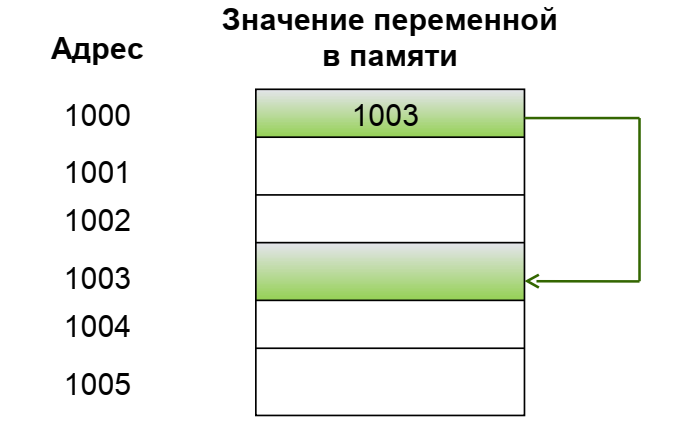
\includegraphics[scale=0.4]{pointer.png}
    \end{figure}
\end{frame}

\begin{frame}{Указательная переменная}
    Объявление указателя состоит из имени базового типа, символа * и имени переменной.
    
    \medskip Общая форма объявления указателя следующая:
    
    \begin{alltt}
    тип *имя;
    \end{alltt}
    
    Здесь \textbf{тип} -- это базовый тип указателя, им может быть любой правильный тип. Имя определяет имя переменной-указателя.
    
    \medskip
    Базовый тип указателя определяет тип объекта, на который указатель будет ссылаться. Фактически указатель любого типа может ссылаться на любое место в памяти. Однако выполняемые с указателем операции существенно зависят от его типа. Например, если объявлен указатель типа \texttt{int *}, компилятор предполагает, что любой адрес, на который он ссылается,
    содержит переменную типа \texttt{int}, хоть это может быть и не так. Следовательно, объявляя указатель, необходимо убедиться, что его тип совместим с типом объекта, на который он будет ссылаться.
\end{frame}

\begin{frame}{Операции для работы с указателями}
    В языке С определены две операции для работы с указателями: \texttt{*} и \texttt{\&}.
    
    Унарная операция \texttt{&} возвращает адрес объекта. Например, операция
    \begin{alltt}
    m = \&count;
    \end{alltt}
    присваивает переменной \texttt{m} адрес переменной \texttt{count}. Можно сказать, что адрес - это номер первого байта участка памяти, в котором хранится переменная. 
    
    \medskip Предположим, переменная \texttt{count} хранится в ячейке памяти под номером 2000, а ее значение равно 100. Тогда переменной m будет присвоено значение 2000.
    
    \medskip Унарная операция * называется операцией ссылки по указателю (indirection) или разыменования (dereferencing). Применяя ее к указателю, получаем объект, на который он указывает. Например, если \texttt{m} содержит адрес переменной \texttt{count}, то оператор
    \begin{alltt}
    q = *m;
    \end{alltt}
    присваивает переменной q значение переменной \texttt{count}. Таким образом, q получит значение 100, потому что по адресу 2000 расположена переменная count, которая имеет значение 100.
\end{frame}

\begin{frame}[fragile]{Операции для работы с указателями}
    \begin{minted}{c}
    int x, *p;
    x = 3;
    p = &x;
    *p = 5;
    \end{minted}
    
    \medskip
    Чему равно значение переменной x?
\end{frame}

\begin{frame}[fragile]{Указательные выражения}
    В выражениях с указателями можно использовать операции присваивания, преобразования типов, а так же сложения и вычитания.
    
    \medskip
    Указатель можно использовать в правой части оператора присваивания для присваивания его значения другому указателю. Если оба указателя имеют один и тот же тип, то выполняется простое присваивание, без преобразования типа:
    \medskip
    \begin{minted}{c}
    int x = 99;
    int *p1, *p2;
    p1 = &x;
    p2 = p1;
    \end{minted}
    \medskip
    
    Оба указателя (\texttt{p1} и \texttt{р2}) ссылаются на \texttt{х}. Допускается присваивание указателя одного типа указателю другого типа.Однако для этого необходимо выполнить явное преобразование типа указателя.
\end{frame}

\begin{frame}{Преобразование типа указателя}
    Указатель можно преобразовать к другому типу. Эти преобразования
    бывают двух видов: с использованием указателя типа \texttt{void *} и без его использования.
    
    \medskip
    В языке С допускается присваивание указателя типа \texttt{void *} указателю любого другого типа (и наоборот) без явного преобразования типа указателя.
    
    \medskip
    Тип указателя \texttt{void *} используется, если тип объекта неизвестен. Например, использование типа \texttt{void *} в качестве параметра функции позволяет передавать в функцию указатель на объект любого типа, при этом сообщение об ошибке не генерируется.
    
    Также он полезен для ссылки на произвольный участок памяти, независимо от размещенных там объектов.
    
    \medskip
    В отличие от \texttt{void *}, преобразования всех остальных типов указателей должны быть всегда явными (т.е. должна быть указана операция приведения типов).
    
    Однако следует учитывать, что преобразование одного типа указателя к другому может вызвать непредсказуемое поведение программы.
\end{frame}

\begin{frame}[fragile]{Преобразование типа указателя}
    В следующей программе делается попытка присвоить значение х переменной у посредством указателя р. При компиляции программы сообщение об ошибке не генерируется, однако результат работы программы неверен.
    \medskip
\begin{minted}{c}
#include <stdio.h>
int main(void) {
    double x = 100.1, y;
    int *p;
    /* В следующем операторе указателю на целое p
    (присваивается значение, ссылающееся на double. */
    p = (int *) &x;
    /* Следующий оператор работает не так, как ожидается. */
    y = *p;
    /* Следующий оператор не выведет число 100.1. */
    printf("Значение x равно: %f (Это не так!)", y);
    return 0;
}
\end{minted}
\end{frame}

\begin{frame}{Адресная арифметика}
    В языке С допустимы только две арифметические операции над указателями: сложение и вычитание.
    
    \medskip Предположим, текущее значение указателя p1 типа int * равно 2000. Предположим также, что переменная типа int занимает в памяти 4 байта. 
    
    \medskip Тогда после операции увеличения
    \mint{c}|p1++;|
    указатель \texttt{p1} принимает значение 2004, а не 2001. То есть, при увеличении на 1 указатель p1 будет ссылаться на следующее целое число.
    
    \medskip Это же справедливо и для операции уменьшения. Например, если p1 равно 2000, то после выполнения оператора
    
    \mint{c}|p1--;|
    
    значение \texttt{p1} будет равно 1996.
\end{frame}

\begin{frame}{Адресная арифметика}
    Операции адресной арифметики подчиняются следующим правилам:
    \begin{itemize}
        \item После выполнения операции увеличения над указателем, данный указатель будет ссылаться на следующий объект своего базового типа.
        \item После выполнения операции уменьшения - на предыдущий объект.
    \end{itemize}
    
    \medskip
    Операции адресной арифметики не ограничены увеличением (инкрементом) и уменьшением (декрементом). 
    
    \medskip Например, к указателям можно добавлять целые числа или вычитать из них целые числа. Выполнение оператора
    \medskip
    \mint{c}|p1 = p1 + 12;|
    \medskip
    "передвигает" указатель \texttt{p1} на 12 объектов в сторону увеличения адресов.
\end{frame}

\begin{frame}{Инициализация указателей}
    После объявления нестатического локального указателя до первого присвоения он содержит неопределенное значение. (Глобальные и статические локальные указатели при объявлении неявно инициализируются нулем.) Если попытаться использовать указатель перед присвоением ему нужного значения, то скорее всего он мгновенно разрушит программу или всю операционную систему. Это очень досадная ошибка.
    
    \medskip
    При работе с указателями большинство программистов придерживаются следующего важного соглашения: указатель, не ссылающийся в текущий момент времени должным образом на конкретный объект, должен содержать нулевое значение. Нуль используется потому, что С гарантирует отсутствие чего-либо по нулевому адресу. Следовательно, если указатель равен нулю, то это значит, во-первых, что он ни на что не ссылается, а во-вторых — что его сейчас нельзя использовать.
\end{frame}

\begin{frame}{Инициализация указателей}
    Указателю можно задать нулевое значение, присвоив ему 0. Например, следующий оператор инициализирует р нулем:
    \medskip
    \mint{c}|char *p = 0;|
    \medskip
    Дополнительно к этому во многих заголовочных файлах языка С, например, в <stdio.h> определен макрос NULL, являющийся нулевой указательной константой. Поэтому в программах на С
    часто можно увидеть следующее присваивание:
    \medskip
    \mint{c}|p = NULL;|
    \medskip
    Однако равенство указателя нулю не делает его абсолютно "безопасным". Использование нуля в качестве признака неподготовленности указателя - это только соглашение программистов, но не правило языка С.
\end{frame}

\begin{frame}[fragile]{Указатели и аргументы функций}
    В языке Pascal существует особый вид параметров функции – var-параметры. Переменным, переданным как var-параметры в функции может быть присвоено новое значение, и это новое значение переменной сохранится после выхода из функции.
    
    \medskip
    В языке С аргументы передаются в функции только по значению, и не существует прямого способа изменить переменную, переданную через параметр функции. Добиться нужного эффекта можно передавая в функцию не саму переменную, а указатель на нее.
    
    \medskip
    В следующем примере показана функция \texttt{swap}, выполняющая обмен значений двух целочисленных переменных:
    
    \medskip
\begin{minted}{c}
void swap(int *px, int *py) /* обмен местами *рх и *ру */
{
    int temp;
    temp = *px;
    *px = *py;
    *py = temp;
}
\end{minted}
    \medskip
    Функция \texttt{swap} вызывается как \texttt{swap(\&a, \&b);}.
\end{frame}

\begin{frame}[fragile]{Указатели и массивы}
    Понятия указателей и массивов тесно связаны. Рассмотрим следующий фрагмент программы:
    \begin{minted}{c}
    char str[80], *p1;
    p1 = str;
    \end{minted}
    
    Здесь \texttt{p1} указывает на первый элемент массива \texttt{str}. Обратиться к пятому элементу массива \texttt{str} можно с помощью любого из двух выражений:
    \begin{minted}{c}
    str[4]
    *(p1+4)
    \end{minted}
    
    Массив начинается с нуля. Поэтому для пятого элемента массива \texttt{str} нужно использовать индекс 4. Можно также увеличить \texttt{p1} на 4, тогда он будет указывать на пятый элемент.
    
    \medskip
    Как и объекты любых других типов, указатели могут быть собраны в массив. В следующем операторе объявлен массив из 10 указателей на объекты типа \texttt{int}:
    \mint{c}|int *x[10];|
    
    Для присвоения, например, адреса переменной \texttt{var} третьему элементу массива указателей, необходимо написать: \qquad \mint{c}|x[2] = &var;|
\end{frame}

\begin{frame}[fragile]{Указатели на функции}
    Указатели на функции – очень мощное средство языка С. Функция
    располагается в памяти по определенному адресу, который можно присвоить указателю в качестве его значения. Адресом функции является ее точка входа. Именно этот адрес используется при вызове функции. Так как указатель хранит адрес функции, то она может быть вызвана с помощью этого указателя. Он позволяет также передавать ее другим функциям в качестве аргумента.
    
    \medskip
    Описание указателя на функцию и вызов функции по указателю показаны ниже. Предполагается, что ранее была описана функция \texttt{max2}, принимающая два аргумента типа \texttt{int} и возвращающее значение типа \texttt{int}.
    
    \medskip
    \begin{minted}{c}
    int a = -5, b = 3, c;
    int (*p)(int, int);/* указатель на функцию */
    p = max2;
    c = (*p)(a,b);/* вызов функции по указателю */
    \end{minted}
    
    \medskip
    При описании указателя на функцию и ее вызове имя функции и знак * необходимо брать в круглые скобки \texttt{(*p)}.
\end{frame}

\begin{frame}[fragile]{Сложные объявления с указателями}
В декларациях обычно используется имя (идентификатор) и один из модификаторов *, [ ] и ( ), причем разрешается использовать более одного модификатора в одной декларации. 
Для раскрытия этих деклараций применяются следующие правила:
\begin{enumerate}
\item Чем ближе модификатор стоит к идентификатору, тем выше его приоритет.
\item Приоритет ( ) и [ ] выше, чем приоритет *.
\item Приоритет повышается заключением в скобки ().
\end{enumerate}

\medskip
\begin{minted}{c}
char **argv
int (*daytab)[13]
int *daytab[13]
void *comp()
void (*comp)()
char (*(*x()) []) ()
char (*(*x[3]) ()) [5]
\end{minted}
\end{frame}

\begin{frame}[fragile]
\begin{minted}{c}
char **argv
/* argv: указатель на указатель на char */

int (*daytab)[13]
/* daytab: указатель на массив[13] типа int */

int *daytab[13]
/* daytab: массив[13] указателей на int */

void *comp()
/* comp: функция, возвращающая указатель на void */

void (*comp)()
/* comp: указатель на функцию, возвращающую void */

char (*(*x()) []) ()
/* x: функция, возвращающая указатель на массив [] 
 * указателей на функцию, возвращающую char */ 
 
char (*(*x[3]) ()) [5]
/* x: массив [З] указателей на функцию, возвращающую 
 * указатель на массив[5] типа char */
\end{minted}
\end{frame}

\section{Динамическое распределение памяти}

\begin{frame}
  \frametitle{Содержание лекции}
  \tableofcontents[current]
\end{frame}

\begin{frame}{Динамическое выделение памяти}
    Указатели используются для динамического выделения памяти
    компьютера для хранения данных. Динамическое распределение означает, что программа выделяет память для данных во время своего выполнения. 
    
    \medskip
    Память, выделяемая в С функциями динамического распределения данных, находится в т.н. динамически распределяемой области памяти (heap). Динамически распределяемая область памяти — это свободная область памяти, не используемая программой, операционной системой или другими программами. Размер динамически распределяемой области памяти заранее неизвестен, но как правило в ней достаточно памяти для размещения данных программы.
    
    \medskip
    Основу системы динамического распределения в С составляют функции
    \texttt{malloc()} и \texttt{free()}. Эти функции работают совместно. Функция \texttt{malloc()} выделяет память, а \texttt{free()} — освобождает ее.
    В программу, использующую эти функции, должен быть включен
    заголовочный файл \texttt{<stdlib.h>}.
\end{frame}

\begin{frame}{Функция \texttt{malloc()}}
    Прототип функции \texttt{malloc()} следующий:
    
    \medskip
    \mint{c}|void *malloc(size_t <<number_of_bytes>>);|
    
    \medskip Здесь \texttt{<<number\_of\_bytes>>} – размер памяти, необходимой для размещения данных. (Тип \texttt{size\_t} определен в \texttt{<stdlib.h>} как некоторый целый без знака.) 
    
    \medskip Функция \texttt{malloc()} возвращает указатель типа \texttt{void *}, поэтому его можно присвоить указателю любого типа.
    
    \medskip
    При успешном выполнении \texttt{malloc()} возвращает указатель на первый байт непрерывного участка памяти, выделенного в динамически распределяемой области памяти. Если в динамически распределяемой области памяти недостаточно свободной памяти для выполнения запроса, то память не выделяется и \texttt{malloc()} возвращает нуль.
    
    При выполнении следующего фрагмента программы выделяется непрерывный участок памяти объемом 1000 байтов:
    \mint{c}|char *p;|
    \mint{c}|p = malloc(1000); /* выделение 1000 байтов */|
    
    После присвоения указатель p ссылается на первый из 1000 байтов
    выделенного участка памяти.
\end{frame}

\begin{frame}[fragile]{Функция \texttt{malloc()}}
    В следующем примере выделяется память для 50 целых чисел. Для повышения мобильности (переносимости программы с одной машины на другую) используется оператор sizeof.

\medskip
\begin{minted}{c}
int *p;
p = malloc(50 * sizeof(int));
\end{minted}

    \medskip
    Поскольку динамически распределяемая область памяти не бесконечна, при каждом размещении данных необходимо проверять, состоялось ли оно. Если \texttt{malloc()} не смогла по какой-либо причине выделить требуемый участок памяти, то она возвращает нуль:
    
     \medskip
\begin{minted}{c}
p = malloc(100);
if(!p) {
    printf("Нехватка памяти.\n");
    exit(1);
}
\end{minted}
\end{frame}

\begin{frame}{Функция \texttt{free()}}
    Функция \texttt{free()} противоположна функции \texttt{malloc()} в том смысле, что она возвращает системе участок памяти, выделенный ранее с помощью функции \texttt{malloc()}.
    
    \medskip
    Функция \texttt{free()} имеет следующий прототип:
    
    \mint{c}|void free(void *p)|
    
    \medskip
    Здесь \texttt{p} — указатель на участок памяти, выделенный перед этим функцией \texttt{malloc()}.
    
    \medskip
    Функцию \texttt{free()} нельзя вызывать с неправильным аргументом, это разрушит всю систему распределения памяти.
\end{frame}

\begin{frame}[fragile]{Пример - динамический массив}
\begin{minted}{c}
#include <stdlib.h>
int main(void)
{
    int *a;
    int i, n = 80;
    
    a = malloc(n*sizeof(int));
    if(!a) {
        printf("Требуемая память не выделена.\n");
        exit(1);
    }
    
    for(i = 0;i < n;i++)
        a[i]=i;
    
    free(a);
    return 0;
}
\end{minted}
\end{frame}

\begin{frame}[fragile]{Трудности при работе с указателями}
    Указатели являются очень мощным средством языка C. В то же время
    неумелое использование указателей может привести к появлению в
    программе нестабильных, труднообнаруживаемых ошибок. Это привело к тому, что в языках-потомках C/С++ (Java, C#) было принято решение отказаться от непосредственной работы с указателями.
    
    \medskip
    Классический пример ошибки – неинициализированный указатель.
\begin{minted}{c}
/* Это программа содержит ошибку. */
int main(void) {
    int x, *p;
    x = 10;
    *p = x; /* ошибка, p не инициализирован */
    return 0;
}
\end{minted}

    \medskip
    Эта программа присваивает значение 10 некоторой неизвестной области памяти.
\end{frame}

\section{Строки}

\begin{frame}
  \frametitle{Содержание лекции}
  \tableofcontents[current]
\end{frame}

\begin{frame}{Строки}
    В языке программирования C отсутствует специальный тип для представления строк, подобный типу string в языке Pascal.
    
    \medskip
    В C строки хранятся как массив символов. При этом размер массива должен быть как минимум на 1 больше числа символов в строке, т.к. после последнего символа строки хранится значение 0, обозначающее конец строки. Отсутствие в конце строки завершающего нуля почти
    наверняка приведет к аварийному завершению программы!
    
    \medskip
    При объявлении строки можно выполнить ее инициализацию строковым
    литералом:
    
    \mint{c}|char s[8] = "example";|
                          
    Данная строка приведет к созданию массива со следующими элементами:
    \begin{tabular}{c c c c c c c c c}
    Элемент & a[0] & a[1] & a[2] & a[3] & a[4] & a[5] & a[6] & a[7]
    \\
    Значение & 'e' & 'x' & 'a' & 'm' & 'p' & 'l' & 'e' & 0
    \end{tabular}
\end{frame}

\begin{frame}{Операции со строками}
    Операции со строками в языке C реализованы с помощью функций,
    находящихся в заголовочном файле \texttt{<string.h>}:
    
    \medskip
    
    \begin{tabular}{|p{3cm}|p{8cm}|}
        \hline
        \textbf{Имя функции} & \textbf{Выполняемое действие} \\ \hline
        \texttt{strcpy(s1, s2)} & Копирование s1 в s2 \\ \hline
        \texttt{strcat(s1, s2)} & Конкатенация (присоединение) s2 в конец s1 \\ \hline
        \texttt{strlen(s1)} & Возвращает длину строки s1 \\ \hline
        \texttt{strcmp(s1, s2)} & Возвращает 0, если s1 и s2  совпадают, отрицательное значение, если s1 < s2 и положительное, если s1 > s2 \\ \hline
        \texttt{strchr(s1, ch)} & Возвращает указатель на первое вхождение символа ch в строку s1 \\ \hline
        \texttt{strstr(s1, s2)} & Возвращает указатель на первое вхождение строки s2 в строку s1\\ \hline
    \end{tabular}
\end{frame}

\begin{frame}[fragile]{Пример работы со строками}
\begin{minted}{c}
#include <stdio.h>
#include <string.h>
int main(void) {
    char s1[80], s2[80];
    gets(s1);
    gets(s2);
    printf("Длина: %d %d\n", strlen(s1), strlen(s2));
    
    if(strcmp(s1, s2)==0) 
        printf("Строки равны\n");
    
    strcat(s1, s2);
    printf("%s\n", s1);
    strcpy(s1, "Проверка.\n");
    printf(s1);
    if(strstr("Привет", "ив")) 
        printf(" найдено ив ");
    
    return 0;
}
\end{minted}
\end{frame}

\section{Структуры}

\begin{frame}
  \frametitle{Содержание лекции}
  \tableofcontents[current]
\end{frame}

\begin{frame}[fragile]{Структуры}
    Структура в языке \textbf{C} представляет собой аналог записи в языке \textbf{Pascal}. Объявление структуры имеет следующий синтаксис:
    \begin{minted}{c}
    struct <<StructureName>> { //имя типа структуры
        <<Fields Definition>> //описание полей
    };
    \end{minted}
    
    В конце описания структуры ставится точка с запятой.
    Описание переменной структурного типа в языке C имеет вид:
    \begin{minted}{c}
    struct StructureName VariableName; 
    \end{minted}
    
    Необходимость указания ключевого слова \texttt{struct} при объявлении структурной переменной является особенностью языка C и отличает его от других языков программирования – C++, Pascal и др.
    
    ~
    
    Доступ к значениям полей структуры осуществляется с помощью операции “.”.
\end{frame}

\begin{frame}[fragile]{Пример работы со структурой}
    \begin{minted}{c}
    struct addr {
        char name[30];
        char street[40];
        char city[20];
        char state[3];
        unsigned long int zip;
    };
    
    struct addr addr_info;
    
    addr_info.zip = 390005;
    \end{minted}
\end{frame}

\begin{frame}[fragile]{Структуры}
    При объявлении структуры можно сразу же объявить одну или несколько переменных структурного типа. 
    
    ~
    
    Например:
    \begin{minted}{c}
    struct addr {
        char name[30];
        char street[40];
        char city[20];
        char state[3];
        unsigned long int zip;
    } addr_info, binfo, cinfo;
    \end{minted}
\end{frame}

\begin{frame}[fragile]{Массивы структур}
    Структуры часто образуют массивы. Чтобы объявить массив структур,
    вначале необходимо определить структуру (то есть определить агрегатный тип данных), а затем объявить переменную массива этого же типа. 
    
    ~
    
    Например:
    
    \mint{c}|struct addr addr_list[100];|
    
    ~
    
    Это выражение создаст 100 наборов переменных, каждый из которых
    организован так, как определено в структуре \texttt{addr}.
    
    ~
    
    Чтобы получить доступ к определенной структуре, нужно указать имя
    массива с индексом. Например, выведем значение ZIP-кода из третьей структуры:
    
\begin{minted}{c}
printf("%d", addr_list[2].zip);
\end{minted}
    
    Как и в других массивах переменных, в массивах структур индексирование начинается с 0.
\end{frame}

\begin{frame}[fragile]{Передача структур функциям}
    Над структурами в целом одного типа можно выполнять операции
    присваивания. Одной из разновидностей такой операции является передача в функцию структурной переменной как аргумента.
    
    ~
    
    В следующем примере вводится структура, описывающая координаты точки и функция, вычисляющая координаты середины отрезка:
\begin{minted}{c}
struct point {
    float x;
    float y;
};

struct point segment_middle(struct point p1, struct point p2)
{
    struct point result;
    result.x = (p1.x + p2.x) / 2;
    result.y = (p1.y + p2.y) / 2;
    return result;
}
\end{minted}
\end{frame}

\begin{frame}{Указатели на структуры}
    В языке C указатели на структуры имеют некоторые особенности.
    
    ~
    
    Чтобы объявить указатель на структуру нужно так же, как и в случае обычных указателей, поместить символ звездочки * перед именем переменной. Например:
    
    \mint{c}|struct addr *addr_pointer;|
    
    ~
    
    Чтобы получить по указателю доступ к полям структуры используется
    операция стрелка “\texttt{->}”:
    
    \mint{c}|addr_pointer->zip = 390000;|
    
    ~
    
    Операции обращения к полям точка и стрелка имеют более высокий
    приоритет, чем остальные. Поэтому в выражении \texttt{++p->len}
    инкрементируется \texttt{len}, а не \texttt{p}.
\end{frame}

\begin{frame}[fragile]{Указатели на структуры}
    В языке C указатели на структуры используются в двух случаях:
    \begin{itemize}
    \item при передаче структуры функции по указателю,
    \item при организации динамических структур данных – списков, очередей, стеков и т.п.
    \end{itemize}
    
    Во втором случае в структуру включается поле – указатель на структуру такого же типа. Заметим, что структура не может содержать в качестве поля структуру такого же типа, а содержать указатель на структуру – может.
    
    ~
    
    Далее описывается возможная структура записи, соответствующей элементу списка:
    
    \begin{minted}{c}
    struct list_item {
        int data[50];
        struct list_item *next;
    };
    \end{minted}
\end{frame}

\begin{frame}[fragile]{Объединения}
    \textbf{Объединение} – это переменная, которая может содержать объекты
    различных типов и размеров (но не одновременно); при этом
    удовлетворение требований к размеру и выравниванию возлагается на
    компилятор. 
    
    ~
    
    С помощью объединений можно работать с данными
    различных типов в пределах одного участка памяти, не привнося в
    программу элементы низкоуровневого, машинно-зависимого
    программирования. 
    
    ~
    
    Объявление объединения (начинается с ключевого слова \texttt{union}) похоже на объявление структуры и в общем виде выглядит так:
    
    \begin{minted}{c}
    union <<Tag>>{
    <<type1>> <<Name1>>;
    <<type2>> <<Name2>>;
    <<type3>> <<Name3>>;
    } <<VariableNamesList>>;
    \end{minted}
\end{frame}

\begin{frame}[fragile]{Объединения}
    Например:
    \begin{minted}{c}
    union u_type {
        int i;
        char ch;
    };
    \end{minted}
    \medskip
    Это объявление не создает никаких переменных. Чтобы объявить
    переменную, ее имя можно поместить в конце объявления или написать отдельный оператор объявления.
    \medskip
    Чтобы с помощью только что написанного кода объявить переменную-объединение, которая называется \texttt{cnvt} и имеет тип \texttt{u\_type}, можно написать следующий оператор:
    \medskip
    \mint{c}|union u_type cnvt;|
    \medskip
    В \texttt{cnvt} одну и ту же область памяти занимают целая переменная \texttt{i} и символьная переменная \texttt{ch}. Конечно, \texttt{i} занимает 2 байта (при условии, что целые значения занимают по 2 байта), a \texttt{ch} — только 1.
\end{frame}

\begin{frame}[fragile]{Битовые поля}
    В языке С имеется встроенная поддержка битовых полей, которая дает возможность получать доступ к единичному биту. Битовые поля могут быть полезны по разным причинам, а именно:
    \medskip
    \begin{itemize}
    \item Если память ограничена, то в одном байте можно хранить несколько булевых переменных (принимающих значения ИСТИНА и ЛОЖЬ);
    \item Некоторые устройства передают информацию о состоянии, закодированную в байте в одном или нескольких битах;
    \item Для некоторых процедур шифрования требуется доступ к отдельным битам внутри байта.
    \end{itemize}
    \medskip
\end{frame}

\begin{frame}[fragile]{Битовые поля}
    Хотя для решения этих задач можно успешно применять побитовые операции, битовые поля могут придать вашему коду больше упорядоченности. 
    
    \medskip
    Битовое поле может быть членом структуры или объединения. Оно определяет длину поля в битах. 
    
    \medskip
    Общий вид определения битового поля такой:
    
    \medskip
    \mint{c}|<<Type>> <<FieldName>> : <<Length>>|
    
    \medskip
    Здесь \texttt{тип} означает тип битового поля, а \texttt{длина} — количество бит, которые занимает это поле. 
    
    \medskip
    Тип битового поля может быть \texttt{int}, \texttt{signed} или \texttt{unsigned}.
\end{frame}

\begin{frame}[fragile]{Битовые поля}
    Например, информацию в байте состояния модема можно представить с
    помощью следующего битового поля:
    
    \begin{minted}{c}
    struct status_type {
        unsigned delta_cts: 1;
        unsigned delta_dsr: 1;
        unsigned tr_edge: 1;
        unsigned delta_rec: 1;
        unsigned cts: 1;
        unsigned dsr: 1;
        unsigned ring: 1;
        unsigned rec_line: 1;
    } status;
    \end{minted}
    
    Для обращения к битовому полю используется тот же способ, что и для обращения к элементу структуры любого другого типа. Вот, например, фрагмент кода, выполняющий сброс поля \texttt{ring}:
    \mint{c}|status.ring = 0;|
\end{frame}

\begin{frame}{Перечисления}
    Перечисление — это набор именованных целых констант. Перечисление в общем виде выглядит так:
    \medskip
    \begin{alltt}
    enum тег \{список\_перечисления\} список\_переменных;
    \end{alltt}
    \medskip
    Здесь \texttt{тег} и \texttt{список\_переменных} не являются обязательными. (Но хотя бы что-то одно из них должно присутствовать.)
    \medskip
    \mint{c}|enum day_of_week { mo, tu, we, th, fr, sa, su };|
    \medskip
    Тег перечисления можно использовать для объявления переменных
    данного перечислимого типа.
    \medskip
    \mint{c}|enum day_of_week today = mo;|
    \medskip
    При задании перечислений одной или нескольким константам можно
    задать связанные с ними значения:
    \medskip
    \mint{c}|enum day_of_week { mo=1, tu=2, we=3, th=4, fr=5, sa=6, su=0 };|
\end{frame}

\begin{frame}{Ключевое слово \texttt{typedef}}
    Новые имена типов данных можно определять, используя ключевое слово \texttt{typedef}. 
    \medskip
    На самом деле таким способом новый тип данных не создается, а всего лишь определяется новое имя для уже существующего типа. Этот процесс может помочь сделать машинно-зависимые программы более переносимыми. Если вы для каждого машинно-зависимого типа данных, используемого в вашей программе, определяете данное вами имя, то при
    компиляции для новой среды придется менять только операторы \texttt{typedef}.
    Такие выражения могут помочь в самодокументировании кода, позволяя давать понятные имена стандартным типам данных.
    Общий вид декларации \texttt{typedef} (оператора \texttt{typedef}) такой:
    
    \begin{alltt}
    typedef тип новое\_имя;
    \end{alltt}
    
    где \texttt{тип} – это любой тип данных языка С, а \texttt{новое\_имя} – новое имя этого типа. Новое имя является дополнением к уже существующему, а не его заменой.
\end{frame}
\end{document}
